\documentclass[journal,12pt,twocolumn]{IEEEtran}

\usepackage{setspace}
\usepackage{gensymb}
\singlespacing
\usepackage[cmex10]{amsmath}

\usepackage{amsthm}

\usepackage{mathrsfs}
\usepackage{txfonts}
\usepackage{stfloats}
\usepackage{bm}
\usepackage{cite}
\usepackage{cases}
\usepackage{subfig}

\usepackage{longtable}
\usepackage{multirow}

\usepackage{enumitem}
\usepackage{mathtools}
\usepackage{steinmetz}
\usepackage{tikz}
\usepackage{circuitikz}
\usepackage{verbatim}
\usepackage{tfrupee}
\usepackage[breaklinks=true]{hyperref}
\usepackage{graphicx}
\usepackage{tkz-euclide}

\usetikzlibrary{calc,math}
\usepackage{listings}
    \usepackage{color}                                            %%
    \usepackage{array}                                            %%
    \usepackage{longtable}                                        %%
    \usepackage{calc}                                             %%
    \usepackage{multirow}                                         %%
    \usepackage{hhline}                                           %%
    \usepackage{ifthen}                                           %%
    \usepackage{lscape}     
\usepackage{multicol}
\usepackage{chngcntr}

\DeclareMathOperator*{\Res}{Res}

\renewcommand\thesection{\arabic{section}}
\renewcommand\thesubsection{\thesection.\arabic{subsection}}
\renewcommand\thesubsubsection{\thesubsection.\arabic{subsubsection}}

\renewcommand\thesectiondis{\arabic{section}}
\renewcommand\thesubsectiondis{\thesectiondis.\arabic{subsection}}
\renewcommand\thesubsubsectiondis{\thesubsectiondis.\arabic{subsubsection}}


\hyphenation{op-tical net-works semi-conduc-tor}
\def\inputGnumericTable{}                                 %%

\lstset{
%language=C,
frame=single, 
breaklines=true,
columns=fullflexible
}
\begin{document}


\newtheorem{theorem}{Theorem}[section]
\newtheorem{problem}{Problem}
\newtheorem{proposition}{Proposition}[section]
\newtheorem{lemma}{Lemma}[section]
\newtheorem{corollary}[theorem]{Corollary}
\newtheorem{example}{Example}[section]
\newtheorem{definition}[problem]{Definition}

\newcommand{\BEQA}{\begin{eqnarray}}
\newcommand{\EEQA}{\end{eqnarray}}
\newcommand{\define}{\stackrel{\triangle}{=}}
\bibliographystyle{IEEEtran}
\raggedbottom
\setlength{\parindent}{0pt}
\providecommand{\mbf}{\mathbf}
\providecommand{\pr}[1]{\ensuremath{\Pr\left(#1\right)}}
\providecommand{\qfunc}[1]{\ensuremath{Q\left(#1\right)}}
\providecommand{\sbrak}[1]{\ensuremath{{}\left[#1\right]}}
\providecommand{\lsbrak}[1]{\ensuremath{{}\left[#1\right.}}
\providecommand{\rsbrak}[1]{\ensuremath{{}\left.#1\right]}}
\providecommand{\brak}[1]{\ensuremath{\left(#1\right)}}
\providecommand{\lbrak}[1]{\ensuremath{\left(#1\right.}}
\providecommand{\rbrak}[1]{\ensuremath{\left.#1\right)}}
\providecommand{\cbrak}[1]{\ensuremath{\left\{#1\right\}}}
\providecommand{\lcbrak}[1]{\ensuremath{\left\{#1\right.}}
\providecommand{\rcbrak}[1]{\ensuremath{\left.#1\right\}}}
\theoremstyle{remark}
\newtheorem{rem}{Remark}
\newcommand{\sgn}{\mathop{\mathrm{sgn}}}
\providecommand{\abs}[1]{\left\vert#1\right\vert}
\providecommand{\res}[1]{\Res\displaylimits_{#1}} 
\providecommand{\norm}[1]{\left\lVert#1\right\rVert}
%\providecommand{\norm}[1]{\lVert#1\rVert}
\providecommand{\mtx}[1]{\mathbf{#1}}
\providecommand{\mean}[1]{E\left[ #1 \right]}
\providecommand{\fourier}{\overset{\mathcal{F}}{ \rightleftharpoons}}
%\providecommand{\hilbert}{\overset{\mathcal{H}}{ \rightleftharpoons}}
\providecommand{\system}{\overset{\mathcal{H}}{ \longleftrightarrow}}
	%\newcommand{\solution}[2]{\textbf{Solution:}{#1}}
\newcommand{\solution}{\noindent \textbf{Solution: }}
\newcommand{\cosec}{\,\text{cosec}\,}
\providecommand{\dec}[2]{\ensuremath{\overset{#1}{\underset{#2}{\gtrless}}}}
\newcommand{\myvec}[1]{\ensuremath{\begin{pmatrix}#1\end{pmatrix}}}
\newcommand{\mydet}[1]{\ensuremath{\begin{vmatrix}#1\end{vmatrix}}}
\numberwithin{equation}{subsection}
\makeatletter
\@addtoreset{figure}{problem}
\makeatother
\let\StandardTheFigure\thefigure
\let\vec\mathbf
\renewcommand{\thefigure}{\theproblem}
\def\putbox#1#2#3{\makebox[0in][l]{\makebox[#1][l]{}\raisebox{\baselineskip}[0in][0in]{\raisebox{#2}[0in][0in]{#3}}}}
     \def\rightbox#1{\makebox[0in][r]{#1}}
     \def\centbox#1{\makebox[0in]{#1}}
     \def\topbox#1{\raisebox{-\baselineskip}[0in][0in]{#1}}
     \def\midbox#1{\raisebox{-0.5\baselineskip}[0in][0in]{#1}}
\vspace{3cm}
\title{EE3025 IDP}
\author{Assignment-1}
\maketitle
\newpage
\bigskip
\renewcommand{\thefigure}{\theenumi}
\renewcommand{\thetable}{\theenumi}
Download all python codes from 
\begin{lstlisting}
https://github.com/Sivanidevarapalli26/EE3025_IDP/tree/main/Assignment-1/Codes
\end{lstlisting}
%
and latex-tikz codes from 
%
\begin{lstlisting}
https://github.com/Sivanidevarapalli26/EE3025_IDP/tree/main/Assignment-1
\end{lstlisting}
\section{Question}
\begin{enumerate}[label=\thesection.\arabic*.,ref=\thesection.\theenumi]
\numberwithin{equation}{enumi}
    
\item Let
\begin{align}
    x(n) = \cbrak{\underset{\uparrow}{1},2,3,4,2,1} \\
    y(n) + \frac{1}{2}y(n-1) = x(n) + x(n-2) \label{eq:1.0.2}
\end{align}
Compute
\begin{align}
    X(k) \triangleq \sum_{n=0}^{N-1}x(n)e^{-j2\pi kn/N},\quad k=0,1, \ldots, N-1
\end{align}
and $H(k)$ using $h(n)$.
\section{Solution}
\begin{enumerate}[label=\thesection.\arabic*.,ref=\thesection.\theenumi]
\numberwithin{equation}{enumi}
\item
When Unit impulse signal is given as input to the LTI system then its impulse response is the ouput of the system.
So,from equation \eqref{eq:1.0.2} we can say that the Impulse response of the system is,
\begin{align}
    h(n) + \frac{1}{2}h(n-1) = \delta(n) + \delta(n-2)	
\end{align}

\item Given that DFT of a Input Signal $x(n)$ is :
\begin{align}
    X(k) \triangleq \sum_{n=0}^{N-1}x(n)e^{-j2\pi kn/N},\quad k=0,1, \ldots, N-1 \label{eq:2.0.2}
\end{align}
\item Similarly, DFT of Impulse Response $h(n)$ is,
\begin{align}
    H(k) \triangleq \sum_{n=0}^{N-1}h(n)e^{-j2\pi kn/N},\quad k=0,1, \ldots, N-1 \label{eq:2.0.3}
\end{align}
\item Python Code to compute the DFT of $x(n)$ and $h(n)$ is given below
\begin{lstlisting}
https://github.com/Sivanidevarapalli26/EE3025_IDP/blob/main/Assignment-1/Codes/ee18btech11012.py
\end{lstlisting}
\item From the above code we get the following plots.
\begin{lstlisting}
https://github.com/Sivanidevarapalli26/EE3025_IDP/tree/main/Assignment-1/figs
\end{lstlisting}
\begin{figure}[h!]
    \centering
    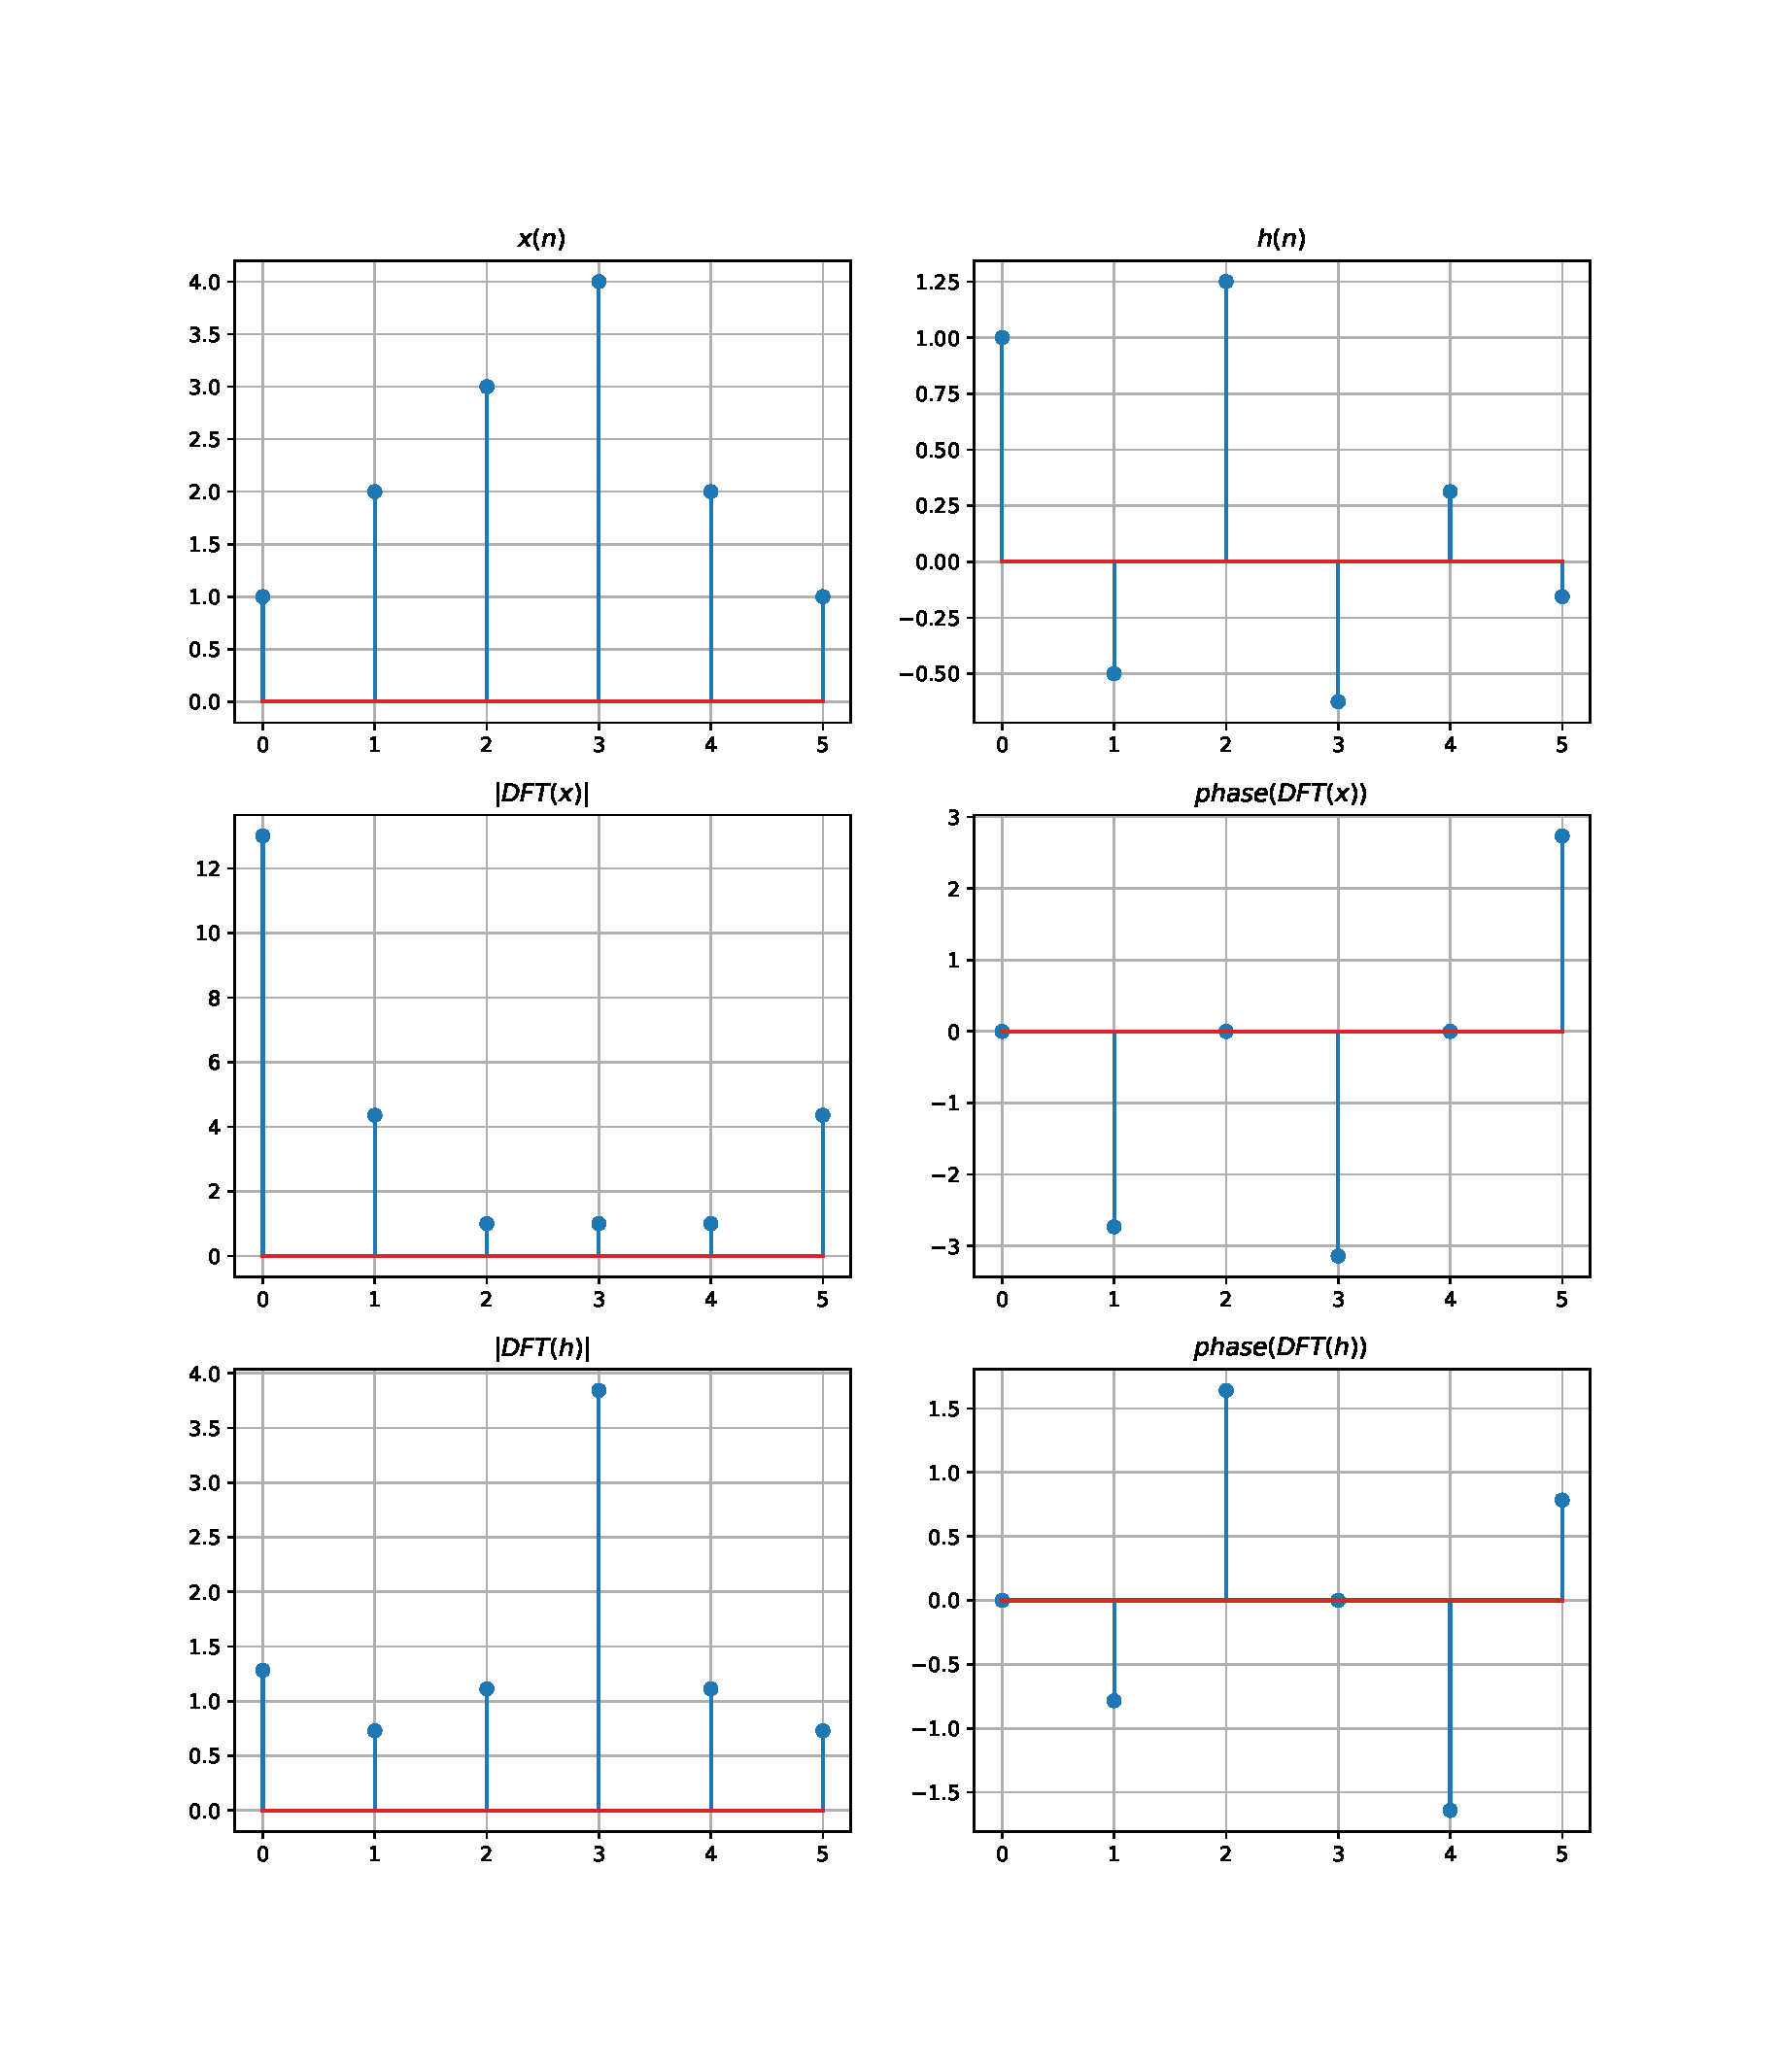
\includegraphics[width=10cm]{ee18btech11012.eps}
    \caption{Plots of x(n) and h(n),their DFTs}
    \label{figs}
\end{figure}


\item
Soving DFT of x(n) and h(n) using Matrix multiplication method
\\
we know that

\begin{align}
    X(k) \triangleq \sum_{n=0}^{N-1}x(n)e^{-j2\pi kn/N},\quad k=0,1, \ldots, N-1
\end{align}
Let $W_N^{nk}=e^{-j2\pi kn/N} $  then this can be expressed interms of matrices as:
\begin{equation}
 \begin{bmatrix} X(0) \\ X(1) \\ X(2) \\ X(3) \\ X(4) \\ X(5) \end{bmatrix}
=
\begin{bmatrix}
1 & 1 & 1 & 1 & 1 & 1 \\ 1 & W_N^1& W_N^2& W_N^3 & W_N^4 & W_N^5\\1 & W_N^2 & W_N^4 & W_N^6 & W_N^8 & W_N^{10}\\1 & W_N^3 & W_N^6 & W_N^9 & W_N^{12} & W_N^{15}\\1 & W_N^4 & W_N^8 & W_N^{12} & W_N^{16} & W_N^{20}\\1 & W_N^5 & W_N^{10} & W_N^{15} & W_N^{20} &W_N^{25}
\end{bmatrix}%
\begin{bmatrix}
x(0) \\ x(1) \\ x(2) \\ x(3) \\ x(4) \\x(5)
\end{bmatrix}

\right
\end{equation}
\item 
Given that  x(n) = \cbrak{\underset{\uparrow}{1},2,3,4,2,1} \\ and As,N=6 then above equation on multiplying matrices  becomes
\begin{equation}
\left
\begin{bmatrix} X(0) \\ X(1) \\ X(2) \\ X(3) \\ X(4) \\ X(5) \end{bmatrix}
=
\begin{bmatrix}
1 +2+3+4+2+1 \\ 1+ (2)e^{-j\pi /3} + ... + (1)e^{-j5\pi /3}\\ 1 + (2)e^{-2j\pi /3} + ... +(1)(e^{-2j5\pi /3}\\ 1 + (2)e^{-3j\pi /3} + ... + (1)e^{-3j5\pi /3}\\ 1 + (2)e^{-4j\pi /3} + ... + (1)e^{-4j5\pi /3}\\ 1 + (2)e^{-5j\pi /3} + ... + (1)e^{-5j5\pi /3}
\end{bmatrix}
\end{equation}
\
\item
On solving we get,
\begin{align}
    \implies X(0) = 13 + 0j,\\
    X(1) = -4 - 1.732j,\\
    X(2) = 1 + 0j,
    \\
    X(3) = -1 + 0j,\\
    X(4) = 1 + 0j,\\
    X(5) = -4 + 1.732j
\end{align}
\item
Now to find $H(k)$ we need to know h(n) first. So we will first calculate h(n). For that we need to first find the Y(z) by applying Z-transform on equation $\eqref{eq:1.0.2}$ i.e.,
\begin{align}
    Y(z) + \frac{1}{2}z^{-1}Y(z)=X(z) + z^{-2}X(z)
\end{align}
\begin{align}
    \implies Y(z)=\frac{2(z^2+1)}{z(2z+1)}X(z)
\end{align}
\
Now we can find H(z) using Y(z)\\
 i.e.,
\begin{align}
    H(z) = \frac{Y(z)}{X(z)}
\end{align}
\begin{align}
 H(z) = \frac{2(z^2+1)}{z(2z+1)}
\end{align}
\begin{align}
 H(z) = \frac{1+z^{-2}}{1+\frac{1}{2}z^{-1}}
\end{align}

From this we can say that h(n) is,
\begin{align}
 h(n)= Z^{-1}\sbrak{\frac{1}{1+\frac{1}{2}z^{-1}} + \frac{z^{-2}}{1+\frac{1}{2}z^{-1}}}
\end{align}
\begin{align}
 h(n)=\sbrak{\frac{-1}{2}}^nu(n) + \sbrak{\frac{-1}{2}}^{n-2}u(n-2)
\end{align}
\
Now for the calculations we can \
 assume that length of h(n) is same as length of x(n) i.e., N = 6.

Similarly Now on solving  equation \eqref{eq:2.0.3} using matrix method for each value of k we get,
\begin{equation}
\left
\begin{bmatrix} H(0) \\ H(1) \\ H(2) \\ H(3) \\ H(4) \\ H(5) \end{bmatrix}
=
\begin{bmatrix}
h(0) + h(1) + h(2) + h(3) + h(4) + h(5) \\h(0) + h(1)e^{-j\pi /3} + ... + h(5)e^{-j5\pi /3}\\h(0) + h(1)e^{-2j\pi /3} + ... + h(5)e^{-2j5\pi /3}\\h(0) + h(1)e^{-3j\pi /3} + ... + h(5)e^{-3j5\pi /3}\\
h(0) + h(1)e^{-4j\pi /3} + ... + h(5)e^{-4j5\pi /3}\\h(0) + h(1)e^{-5j\pi /3} + ... + h(5)e^{-5j5\pi /3}
\end{bmatrix}
\end{equation}
\item
On solving we get,
\begin{align}
\implies H(0) = 1.28125 + 0j,\\
 H(1) = 0.51625 - 0.5141875j,\\
 H(2) = -0.078125 + 1.1095625j,\\
 H(3) = 3.84375 + 0j,\\
 H(4) = -0.071825 - 1.1095625j.\\
 H(5) = 0.515625 + 0.5141875j
\end{align}
So,These values which we got are same as that of from the plots.
\
\end{document}
